\begin{figure}[!b]
\begin{center}
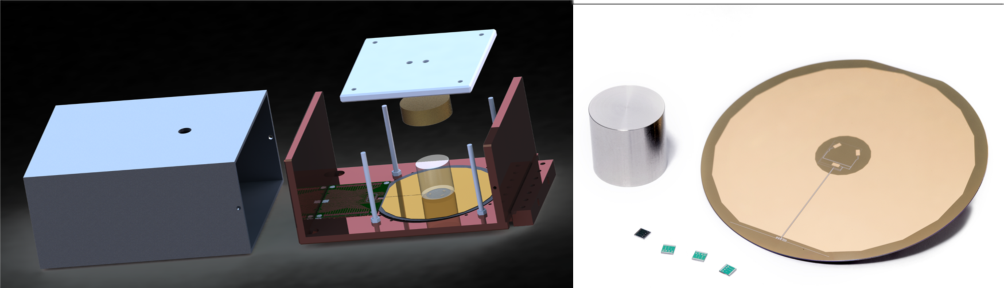
\includegraphics[width=\textwidth]{./fig/Antrag-DELight-extract.pdf}
\vspace{-0.5cm}
\caption{Links: Schema des DELight Aufbaus mit dem zylinderförmigen Detektor auf den drei MMCs und der entsprechenden Halterung inklusive der Vakuum Kupferelektrode. Rechts: Germaniumkristall, dreieckige MMC Struktur und SQUID-holding Chips.}
\label{fig:DELightAufbau}
\end{center}
\end{figure}
\todo{CITE SCHEMATIC \ref{fig:DELightAufbau}}
Bei einer DM-Elektron Streuung entsteht eine bestimmte Anzahl Elektron-Loch-Paare im Germanium Target.
Diese soll bestimmt werden, da sie Aufschluss über die deponierte Energie gibt.
Dazu wird über eine Elektrode ein Potential im Kristall erzeugt, wodurch die Ladungsträger anfangen zu driften.
Dadurch entstehen zwei Signale, welche gemessen werden können.
Erstens induzieren die driftenden Ladungsträger ein Strom in nahegelegenen Elektroden gemäß dem Shockley-Ramo-Theorem\cite{Ramo1939}(siehe Abschnitt \ref{sec:Ramo}), welcher über einen Ionisationskanal gemessen werden kann.
Zweitens erzeugen die Ladungsträger beim Driften sekundäre Phononen, was als Neganov-Luke-Effekt\cite{Luke1988} (siehe Abschnitt \ref{sec:LukeAmp}) bezeichnet wird.
Die Anzahl der Phononen hängt von dem durchlaufenen Potential ab und kann daher im Prinzip beliebig groß gewählt werden.
Dies wird als Luke-Verstärkung bezeichnet.
Primär soll das Ionisationssignal im Wärmekanal ausgelesen werden.
Dazu werden  \acp{MMC}\cite{Fleischmann2009, Enss2005} verwendet, welche eine ausgezeichnete Energieauflösung aufweisen.
Das Ionisationssignal soll trotz schlechterer Auflösung auch über einen Ionisationskanal ausgelesen werden.
Allerdings nicht um Signale DM zu messen sondern um für große Signale (z.B. einer radioaktiven Quelle) die theoretisch erwartete Luke-Verstärkung zu überprüfen.

In Abb.\ref{fig:DELightAufbau} ist das Schema des Aufbaus dargestellt.
Der zylinderförmige Detektor steht auf einer dreieckigen Anordnung von MMCs.
Statt aufgedampften Elektroden wie sie EDELWEISS verwendet sorgt eine Vakuum separierte Elektrode für das notwendige Potential für die Luke-Verstärkung.
Die Vakuum separierte Elektrode hat den Vorteil, dass der Detektor ausschließlich über die MMCs mit dem externen Wärmebad gekoppelt ist und somit kein Wärmesignal durch Kabel der Elektrode verloren gehen.
Außerdem kommt es nicht zu Strömen an der Oberfläche, welche Signale erzeugen und die Wärmekapazität der Elektrode trägt nicht zur gesamten Wärmekapazität des Detektors bei.
Ein Nachteil ist allerdings, dass ein Teil des angelegten Potentials am Vakuumspalt abfällt und somit nur ein Teil des Potentials für die Ladungsträger zum Durchlaufen zur Verfügung steht.
Der genaue Verlauf des Potentials im Detektor ist Gegenstand aktueller Untersuchungen.


